\documentclass[a4paper,11pt]{jreport}

% ------------------------------------------------------------
% usepackage
% ------------------------------------------------------------
\usepackage{sie-jp}
\usepackage{times}
\usepackage{url}
\usepackage{cite}
\usepackage{float}
\usepackage{here}
\usepackage{color}
\usepackage{xcolor}
\usepackage[dvipdfmx]{graphicx}
\usepackage[dvipdfmx,setpagesize=false,bookmarks=true,bookmarksnumbered=true,bookmarkstype=toc]{hyperref}
\usepackage{pxjahyper}
\usepackage{booktabs}
\usepackage{amsthm}
\usepackage{amsmath}
\usepackage{amsfonts}
\usepackage{algorithm}
\usepackage{algorithmicx}
\usepackage{algpseudocode}
\usepackage{listings}
\usepackage{subcaption}
\usepackage{svg}
\usepackage{paralist}
\usepackage{multirow}
\usepackage{todonotes}


% ------------------------------------------------------------
% set
% ------------------------------------------------------------
\setcounter{tocdepth}{3}
\setcounter{page}{-1}
\setlength{\oddsidemargin}{0.1in}
\setlength{\evensidemargin}{0.1in}
\setlength{\topmargin}{0in}
\setlength{\textwidth}{6in}
\setlength{\parskip}{0em}
\setlength{\topsep}{0em}

% ------------------------------------------------------------
% macro
% ------------------------------------------------------------
\renewcommand{\bibname}{参考文献}
\newcommand{\argmax}{\mathop{\rm arg~max}\limits}
\newcommand{\argmin}{\mathop{\rm arg~min}\limits}
\theoremstyle{definition}
\newtheorem{theorem}{定理}
\newtheorem*{theorem*}{定理}
\newtheorem{definition}[theorem]{定義}
\newtheorem*{definition*}{定義}
\renewcommand\proofname{\bf 証明}

% ------------------------------------------------------------
% Packages
% ------------------------------------------------------------
\lstset{
      language=C,
      basicstyle=\footnotesize,
      commentstyle=\textit,
      classoffset=1,
      keywordstyle=\bfseries,
      frame=tRBl,framesep=5pt,
      showstringspaces=false,
      numbers=left,stepnumber=1,numberstyle=\footnotesize
}

% ------------------------------------------------------------
% document
% ------------------------------------------------------------

\begin{document}

% ------------------------------------------------------------
% Title & Abstract & ListOfContents
% ------------------------------------------------------------

\title{筑波大学大学院理工情報生命学術院システム情報工学研究群における修士論文の書き方}
\author{筑波 太郎}
\degree{修士(○○○○)}
\advisor{筑波 大二郎}
\majorfield{△△△△} \programfield{□□□□} \yearandmonth{20XX年 3月}

\maketitle
\thispagestyle{empty}
\newpage
\thispagestyle{empty}
\vspace*{20pt plus 1fil}
\parindent=1zw
\noindent

% textlint-disable
\begin{center}
    {\bf 概要}
    \vspace{5mm}
\end{center}

この文書は,筑波大学大学院システム情報工学研究科の修士論文本体のサンプル
である.このファイルを書き換えて,この例と同じような書式の論文本体を
\LaTeX を使って作成することができる.

このサンプルは,学生諸君が面倒な位置決めをして表紙を作成する手間を軽減す
るために提供している.もちろん,このサンプルで示す表紙は例であり,要項に
準拠していれば,このファイルに頼らずに自分で表紙の位置決めを行ってもよい.
% textlint-enable

\vspace{10mm}

加えて,このリポジトリはシステム情報工学研究科の修士論文本体のサンプルをカスタマイズしたものです.
いくつかの機能ならびに変更を追加しています.
よって,テンプレートにおけるすべての権利はシステム情報工学研究郡に帰属します.

\vspace{0pt plus 1fil}
\newpage

\pagenumbering{roman}
\tableofcontents
\listoffigures
\listoftables
\listoftodos

\pagebreak
\setcounter{page}{1}
\pagenumbering{arabic}

% ------------------------------------------------------------
% Introduction
% ------------------------------------------------------------

\chapter{はじめに}
修士論文自体は,まとめて製本し保存するため,体裁を大体そろえてもらうこと
になっている.そのため,このような修士論文本体の形式の例を作成した.

研究の内容や分野によっては書き方が異なる場合もあるので,詳しいことは指導教員に聞くと
よい.この文書は主にタイトルの作成方法と,論文の体裁を示すのみであり,どうやっ
たらよい論文になるかの示唆は含まれていない.
\section{カスタマイズ}

これ以降,``tsukuba-mas'' にあるオリジナルリポジトリ ``master\_report\_template'' を $A$ と呼びます.
また,$A$ のリポジトリを,あなたの GitHub リポジトリ に ``fork'' もしくは ``import'' したものを $B$ とします.
$B$ のリポジトリであなたの論文を書いていくことになります.

$A$ は,以下 URL で示されている学位論文テンプレートをカスタマイズしたものです.
よって,テンプレートにおけるすべての権利はシステム情報工学研究郡に帰属します.

\url{https://www.sie.tsukuba.ac.jp/visitor/student/thesis_after2020}

具体的には,以下のような変更が加えられています.

\begin{itemize}
    \item UTF-8 対応
    \item GitHub Actions 自動ビルド
    \item Make タスクツール
    \item textlint による自動校正
    \item components ファイル分割
\end{itemize}

\subsection{Clone}

あなたの論文をかくときには,$A$ のリポジトリを fork または import して
あなたのリポジトリに $B$ として追加してください.

論文を書く場合のおすすめは,import です.
$A$ に修正や機能追加などをする場合は,fork して PR を投げてもらえればうれしいです.

\begin{figure}[H]
    \centering
    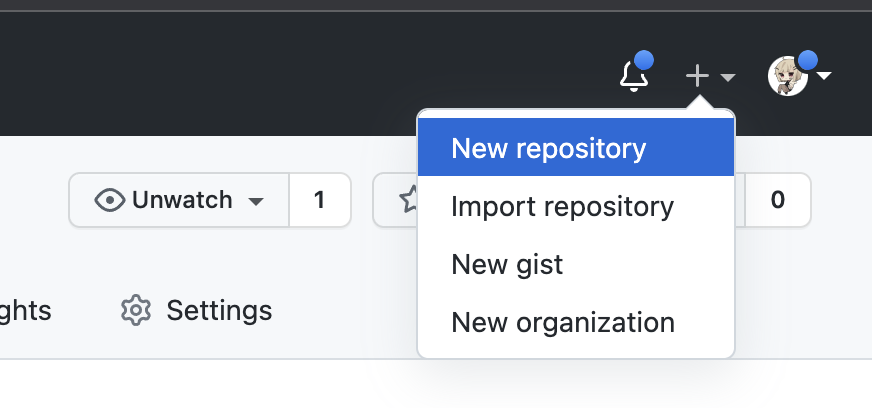
\includegraphics[width=0.5\linewidth]{static/introduction/import.png}
    \caption{$A$ を import する場合.}
\end{figure}

\subsection{GitHub Actions}

$A$ および $B$ には GitHub Actions が設定されています.
($A$ に設定されている GitHub Actions がそのまま $B$ にコピーされるためです.)
基本的な機能については,以下 2 つの記事で紹介しています.

\url{https://zenn.dev/ganariya/articles/platex-github-action}

\url{https://zenn.dev/ganariya/articles/weekly-paper-trial}

以下のような機能がついています.

\begin{itemize}
    \item Pull Request 時に textlint (後述) で文章校正テストを行う
    \item Git Tag を Push すると自動ビルドする
    \item 毎週決まった時間に自動ビルドする
    \item ビルド結果を Slack に通知する
\end{itemize}

ただし,Slack の機能を動作させるためには,$B$ のリポジトリで追加の設定が必要です.
\todo{Webhook URL の箇所が分かりづらいかも}
図\ref{fig:introduction_secrets}が示すように, ``Slack Webhook Incoming'' の URL を GitHub の Secrets に保存する必要があります.

\begin{figure}[H]
    \centering
    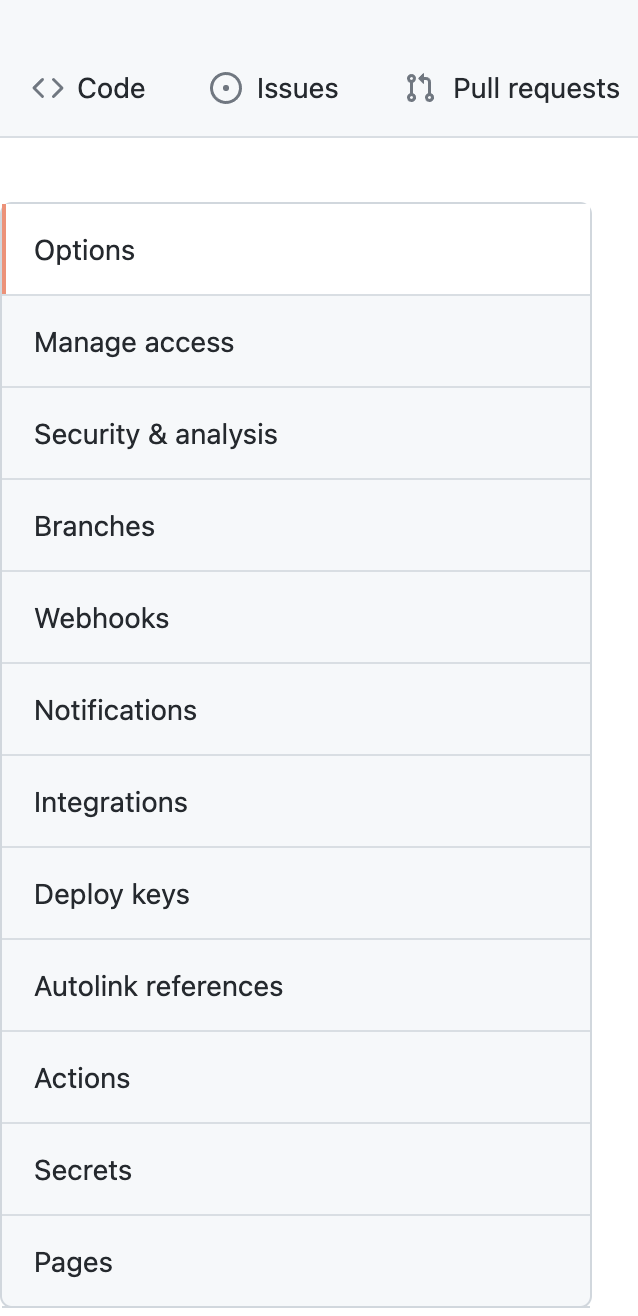
\includegraphics[width=0.3\linewidth]{static/introduction/secrets.png}
    \caption{GitHub Secrets}
    \label{fig:introduction_secrets}
\end{figure}

図\ref{fig:introduction_slack_webhook}が示すように,``SLACK\_WEBHOOK'' キーに,Webhook Incoming の URL を設定してあげてください.

\begin{figure}[H]
    \centering
    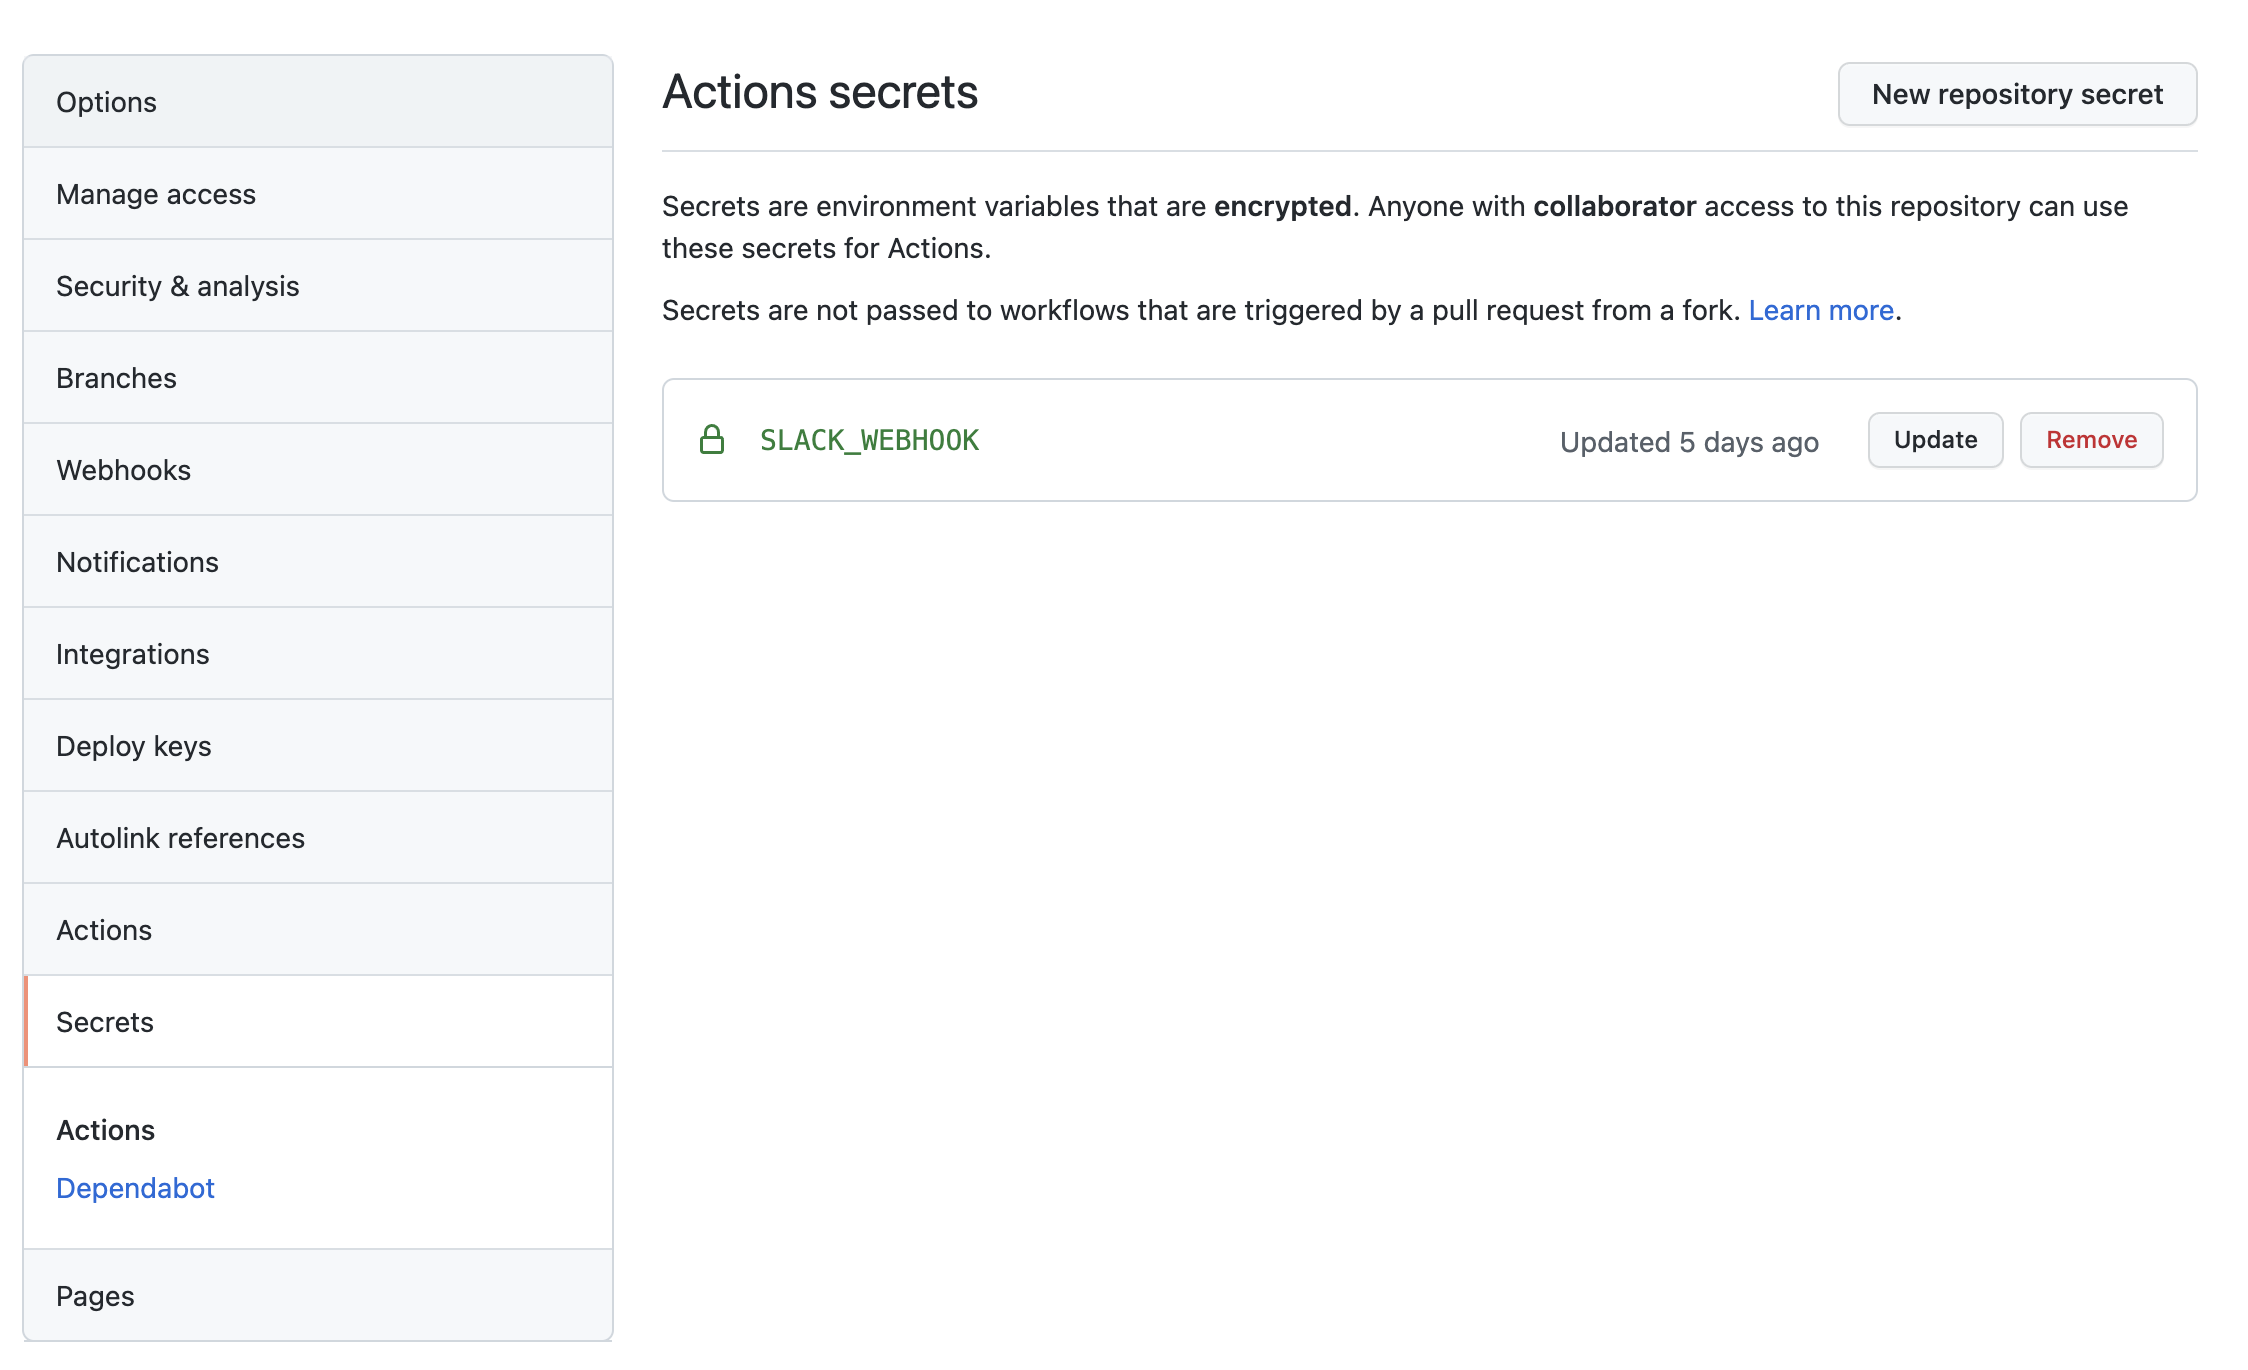
\includegraphics[width=0.6\linewidth]{static/introduction/slack_webhook.png}
    \caption{SLACK WEBHOOK}
    \label{fig:introduction_slack_webhook}
\end{figure}

\subsection{make}

Makefile が用意されています.
そのため,以下のようにコマンドを打つとコンパイルなどの処理が行えます.

とくに,textlint の機能を使うためには make install する必要があります.
make で行っている具体的な処理については Makefile を見てみてください.

\begin{lstlisting}[language=bash,caption={Makefile}]
# Install
make install

# compile
make compile

# clean
make clean
\end{lstlisting}

\subsection{textlint}

textlint というツールは,文章を自動校正してくれます.
自動校正の設定については,``.textlintrc'' で設定されています.
このファイルを変更することで,文章自動校正の設定を変更できます.

自動校正したいときは,``make lint'' などをすると良いです.
``make fix-lint'' することで,治せる部分は textlint が自動で修正してくれます.

ただし,textlint を使うためには,あらかじめ ``make install'' してください.
実質的には, ``npm install'' をしています.

\subsection{Welcome for Your Contributes}

% textlint-disable
修正や機能追加などのプルリクエストをお待ちしています!
% textlint-enable

% ------------------------------------------------------------
% Introduction
% ------------------------------------------------------------

\chapter{形式}
ここでは,論文の表紙および本体の記述方法について述べる.

\section{表紙}

表紙は,{\tt $\backslash$maketitle} によって作成するため,以下の項目に相
当する文字列をそれぞれ記述する.

% textlint-disable
\begin{description} \parskip=1pt
    \item{題目: }
          題目は{\tt $\backslash$title} に記述する.行替えを行う場合は$\backslash$
          $\backslash$ を入力する.ただし,題目の最後に$\backslash$
          $\backslash$ を入力するとコンパイルが通らなくなるので注意する.
          なお,4行以上の題目の場合,表紙ページがあふれるためスタイルファ
          イル``sie-euc.sty''を変更する必要がある.
    \item{著者名: }
          著者名は{\tt $\backslash$author} に記述する.
    \item{学位: }
          学位名は{\tt $\backslash$degree} に記述する.
    \item{指導教員名: }
          指導教教員は{\tt $\backslash$advisor} に記述する.
    \item{専攻名: }
          専攻名は{\tt $\backslash$majorfield} に記述する.
    \item{学位プログラム名: }
          学位プログラム名は{\tt $\backslash$programfield} に記述する.
    \item{年月: }
          年月は{\tt $\backslash$yearandmonth} に記述する.
\end{description}
% textlint-enable
\section{本体}

本体は1段組で記述する.

詳しくは参考書など(少し古い)\cite{野寺隆志1990楽々}\cite{磯崎秀樹1992latex}を参照のこと.
また,奥村晴彦氏の「日本語\TeX 情報(Japanese TeX FAQ)」
\url{http://www.matsusaka-u.ac.jp/~okumura/texfaq/} は,日本語の \TeX に関す
る情報が充実している.くわえて,具体的な論文としての文献参照例として
\cite{bryant1986graph}を挙げておく.


% ------------------------------------------------------------
% Acknowledgement
% ------------------------------------------------------------

\chapter*{謝辞}
\addcontentsline{toc}{chapter}{\numberline{}謝辞}
\newpage
% ------------------------------------------------------------
% Bibliography
% ------------------------------------------------------------

\addcontentsline{toc}{chapter}{\numberline{}参考文献}
\bibliographystyle{junsrt}
\bibliography{related}

\end{document}
